\documentclass[twocolumn]{article}
\usepackage[english]{babel}
\usepackage[utf8]{inputenc}
\usepackage{amsmath,amssymb,physics,mathtools,blindtext,graphicx}
\usepackage[a4paper,total={7.5in,10in}]{geometry}
\usepackage[labelfont=bf]{caption}

\begin{document}
\begin{large}
\section*{Eigenstates of a modified harmonic oscillator}
\subsection*{Introduction}
In quantum mechanics, one is often interested in solving the stationary Schrödinger equation in one dimension:
\begin{equation}
    -\frac{\hbar^2}{2m}u''(x) + V(x)u(x) = Eu.
\end{equation}
This equation can be viewed as an eigenvalue problem $\mathcal{H}u = Eu$ where $\mathcal{H}$ is the hamiltonian given above. The solution $u$ can then be approximated by finding the eigenvalues of the discretized Hamiltonian $H$. In this report, a description will be given on how such an eigenvalue problem can be solved using the inverse power method. The result of applying this method on the following modified harmonic oscillator potential will then be presented.
\begin{equation}
    \label{5apr0811}
    \begin{split}
        &V(x) = \frac{m\omega^2x^2}{2}+\frac{\alpha\hbar\omega}{2}e^{-x^2m\omega/\hbar} - A(\alpha).
    \end{split}
\end{equation}
The constant $A$ makes sure that the lowest point of the potential is zero. This reduces to the harmonic oscillator potential for $\alpha=0$. 

\subsection*{Discretizing the hamiltonian}
We will first consider a general potential $V$ and write the Schrödinger equation in the dimensionless form
\begin{equation}
    \label{2apr1953}
    -u''(\xi) + V(\xi)u(\xi) = E'u(\xi)
\end{equation}
where we assume square integrable solutions $u$ on the real line and that $u(|\xi|\to\infty) = 0$. In order to discretize the hamiltonian, we introduce the gridpoints $\xi_j$ and the approximations of the function $u$ at these gridpoints, $u_j\approx u(\xi_j)$. The step size $h=\xi_{j+1}-\xi_j$ is assumed to be constant. Furthermore, we assume that $\xi_j\in[-L,L]$, where $L$ is chosen such that $u(\xi)\approx 0$ for $|\xi|\geq L$. The second derivative in the hamiltonian is discretized using finite differences and the potential term is discretized in a straightforward manner: $V(\xi_j)u_j$. More details on this is given in an appendix. Using the discretizations, and the fact that $u_j=0$ for large enough $|j|$, the eigenvalue equation $H\mathbf{u} = E\mathbf{u}$ can be set up, where $u_j$ are the elements of $\mathbf{u}$. 
%\begin{equation}
%    H = \frac{1}{12h^2}\left(
%        \begin{matrix}
%            30+12h^2V(\xi_j)  & -16 & 1 & 0 & \dots \\ 
%            -16 & 30 & -16 & 1 & \dots \\ 
%            30 & -16 & 1 & 0 & \dots \\ 
%        \end{matrix}\right)
%\end{equation}

Another approach, which could be used for symmetric potentials, is to assume that the solutions are either even or odd and disregard the negative axis and impose the following boundary conditions:
\begin{equation}
    \begin{rcases}
        &u'(0) = 0 \quad \text{for even } u, \\ 
        &u(0) = 0  \quad \text{for odd } u.
    \end{rcases}
\end{equation} 
%\begin{equation}
%    \begin{split}
%        &u'(0) = 0 \quad\text{and}\quad u(L) = 0 \quad \text{for even } u, \\ 
%        &u(0) = 0 \quad\text{and}\quad u(L) = 0 \quad \text{for odd } u.
%    \end{split}
%\end{equation} 
This will result in two different discretizations of the hamiltonian, $H_\text{even}$ and $H_\text{odd}$, corresponding to these two different boundary conditions. 

%There could however exist eigenstates which vanish at the origin and that have derivatives which also vanish at the origin. In that case it is a eigenstate of both $H_\text{even}$ and $H_\text{odd}$ and special care has to be taken in determining whether the function should be even or odd. When finding the lowest energies, this isn't such a big problem because the ground state is even and all higher energy states alternate between being even and odd with increasing energy.

Having set up the eigenvalue problem $H\mathbf{u} = E\mathbf{u}$ one can search for eigenvectors and eigenvalues by iteratively solving $(H-E'I)\mathbf{u}_{j+1} = \mathbf{u}_j$ and normalizing $\mathbf{u}_j$ in each step. Here $I$ is the identity matrix and $E'$ is a guess at some eigenvalue. The approach which was taken in order to find the states of the modified harmonic oscillator, was to begin with finding the lowest energy state, $E_1$, with $H_\text{even}$, use a new slightly higher guess for the first excited state $E_2$ and iterate with $H_\text{odd}$, then use a slightly higher guess for the second excited state $E_3$ and iterate with $H_\text{even}$ etc. In the following results, the initial guess for the eigenvector was a random vector and the stopping criterion for the iteration was $|H\mathbf{u}-E'\mathbf{u}|_\text{max}<10^{-6}$. 
%The eigenstates, ordered with increasing energy $E_0<E_1<E_2<\dots$, can then be approximated by solving the eigenvalue problems:
%However, with the fourth order approximation used, the difference is only in the first two rows (more details on how these two matrices were constructed are given in an appendix).
%\begin{equation}
%    \begin{split}
%        &H_\text{even}\mathbf{u}_0 = E_0\mathbf{u}_0 \\ 
%        &H_\text{odd } \mathbf{u}_1 = E_1\mathbf{u}_1 \\ 
%        &H_\text{even}\mathbf{u}_2 = E_2\mathbf{u}_2 \\ 
%        &H_\text{odd }\mathbf{u}_3 = E_3\mathbf{u}_3 \\ 
%        &\hspace{1.5cm} \vdots
%    \end{split}
%\end{equation}


\subsection*{Results}
%The stationary Schrödinger equation for the harmonic oscillator is 
%\begin{equation}
%    -\frac{\hbar}{2m}u''(x) + \frac{m\omega^2}{2}x^2 = Eu
%\end{equation}
By changing the variables with $\xi = x/\sqrt{\hbar/m\omega}$ and $E' = 2E/\hbar\omega$, the potential \eqref{5apr0811} can be written in the form of \eqref{2apr1953} where the potential is  
\begin{equation}
    \label{29mar1748}
    V(\xi) = \xi^2+\alpha e^{-\xi^2} - A(\alpha).
\end{equation}
\begin{figure}[b!]
    \centering
    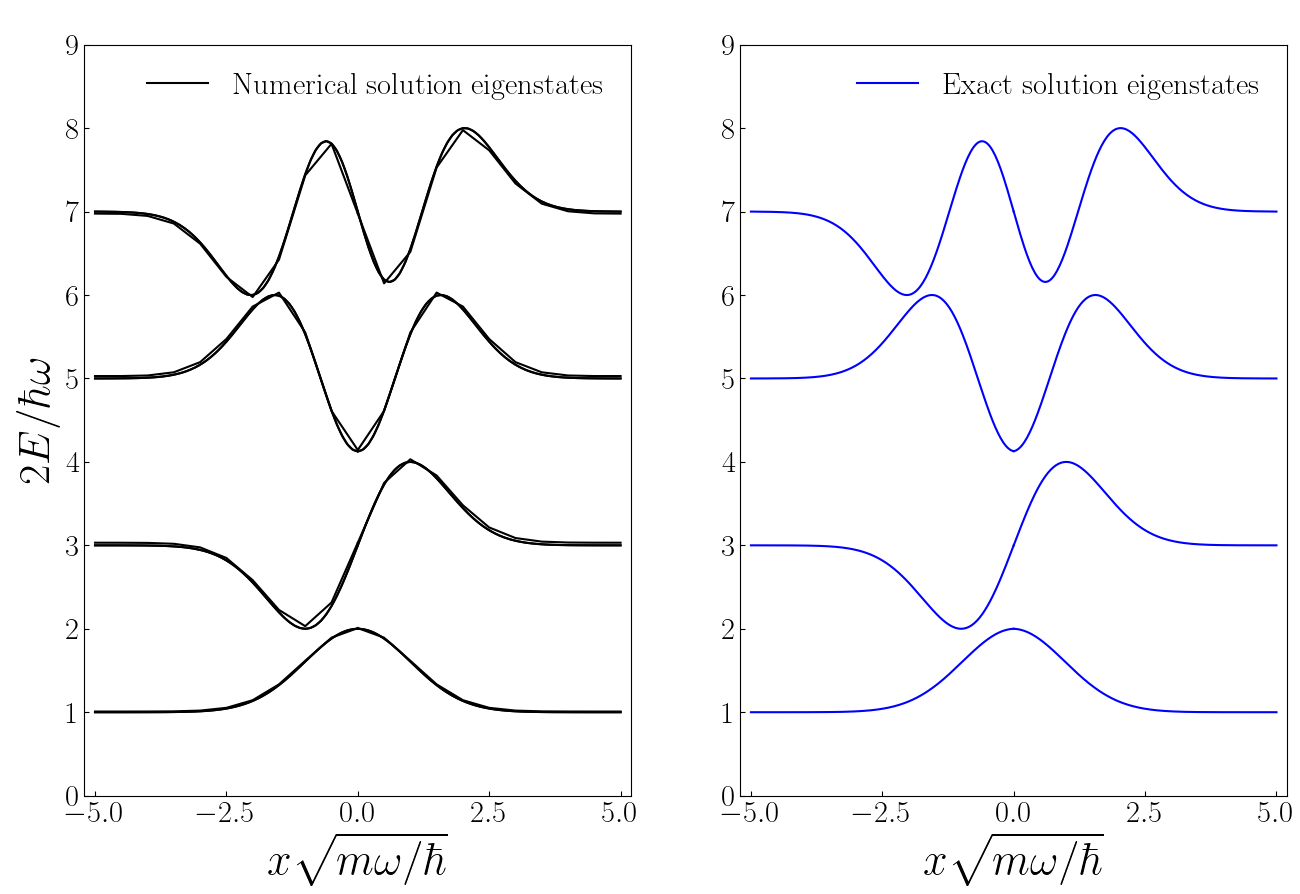
\includegraphics[scale=0.28]{comparison.png}
    \caption{Comparison between exact solutions and numerical solutions using the inverse power method for the quantum harmonic oscillator. The step sizes used in the numerical solution above were $h=0.025$, $0.1$ and $0.5$.}
    \label{2apr2208}
\end{figure}
For $\alpha=0$, this becomes the potential for a quantum harmonic oscillator. In these reduced units, its eigenvalues are known to be $E'=1,3,5,7,\dots$. This gives us a way to test the validity of the method.
The inverse power iteration worked quite well on the quantum harmonic oscillator. A run over the first 150 eigenstates gave a maximum deviation of 0.03 (in reduced units) from the true energy value. The first four eigenstates are plotted in figure \ref{2apr2208} along with the exact solutions. The numerical solution seems to agree well with the exact solution even for quite large step sizes ($h=0.5$). The number of power iterations necessary to reach the error tolerance was never above 100.

The probability density for the first couple of eigenstates for $\alpha=0$ (i.e. the harmonic oscillator) can be seen in figure \ref{4apr0717}. The step size used here and in all subsequent results was $h=0.025$. As can be seen in the figure, with each energy level, the number of nodes increases by one and the wavefront gets shifted further away from the origin. The relationship between the energy levels and the distance of wavefront from the origin, $D$, was further investigated (see figure \ref{4apr1941}). For large energies $E$, this relationship becomes $D\sim\sqrt{E}$ which is the same relationship between the energy and the maximum displacement of the classical harmonic oscillator.
\begin{figure}[b!]
    \centering
    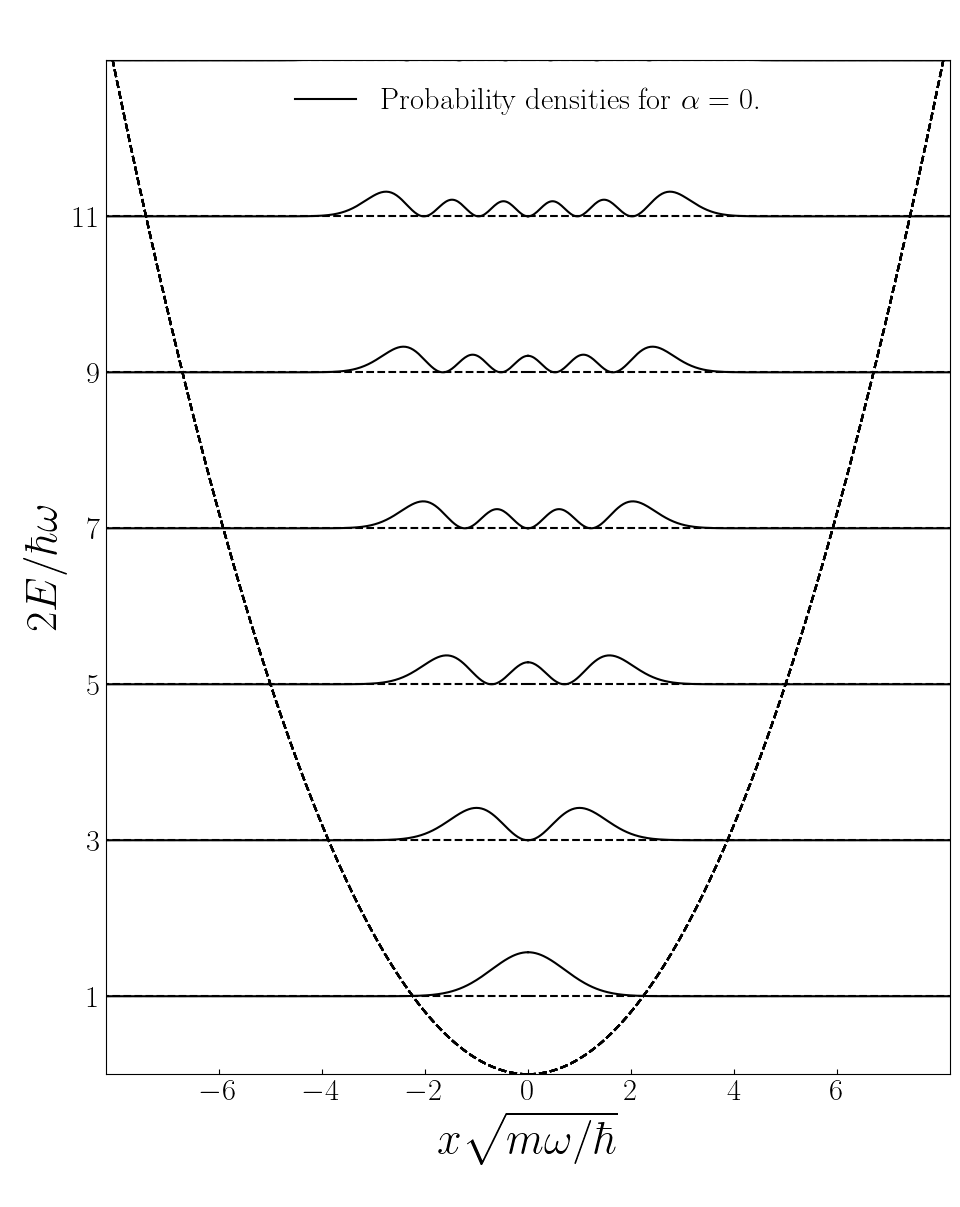
\includegraphics[scale=0.36]{har_osc_density.png}
    \caption{The first couple of probability densities for the harmonic oscillator ($\alpha=0$) obtained with power iteration.}
    \label{4apr0717}
\end{figure}

\begin{figure}[t!]
    \centering
    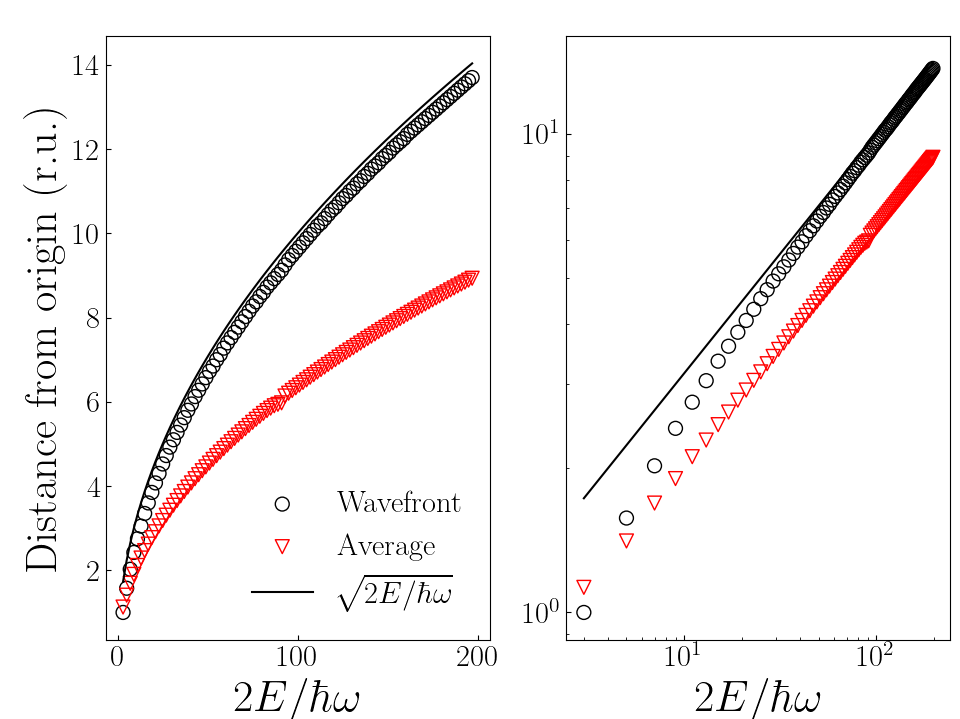
\includegraphics[scale=0.35]{dist.png}
    \caption{The distance of the wavefront and the average distance from the origin as a function of energy.}
    \label{4apr1941}
\end{figure}
\begin{figure}[b!]
    \centering
    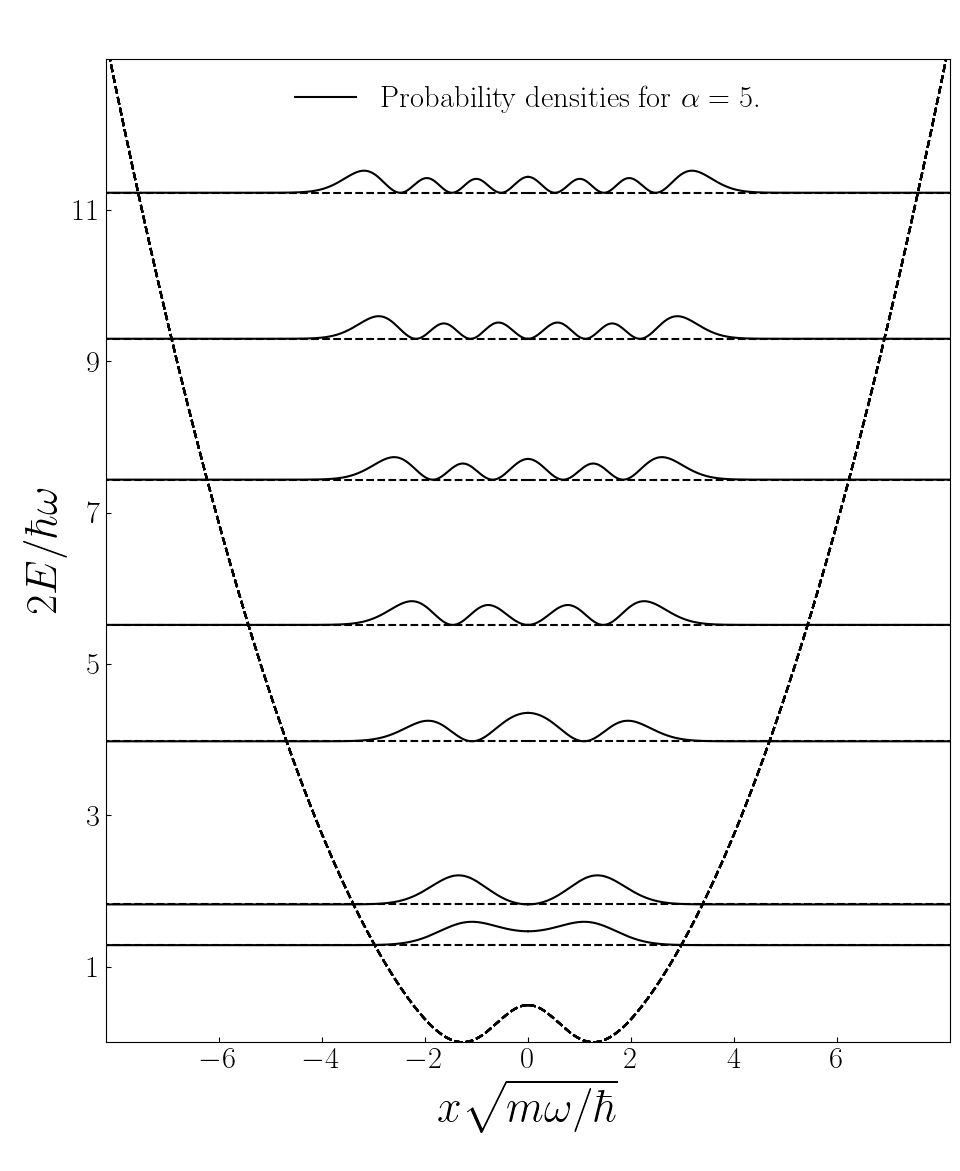
\includegraphics[scale=0.37]{alpha5_density.png}
    \caption{The first couple of probability densities for the modified harmonic oscillator with $\alpha=5$.}
    \label{4apr2003}
\end{figure}
The power iteration method was then tested for $\alpha=5$ and $\alpha=10$. The probability densities for the first couple of eigenstates can be seen in figures \ref{4apr2003} and \ref{4apr2029}. The first two eigenstates are plotted in figure \ref{5apr0727}. A major difference to the harmonic oscillator are the spacings between the first two eigenstates. For $\alpha=5$, the difference was $E'_2-E'_1 = 0.54$ and for $\alpha=10$, $E'_2-E'_1 = 0.08$. The spacings then seem to vary less for higher energy which is better shown in figure \ref{4apr2044}. This reflects the fact that for large $E$, the $\sim e^{-\xi^2}$ part of the Schrödinger equation has less effect and the eigenstates begin to look like harmonic oscillator states. Figure \ref{4apr2029} demonstrates this.
\begin{figure}
    \centering
    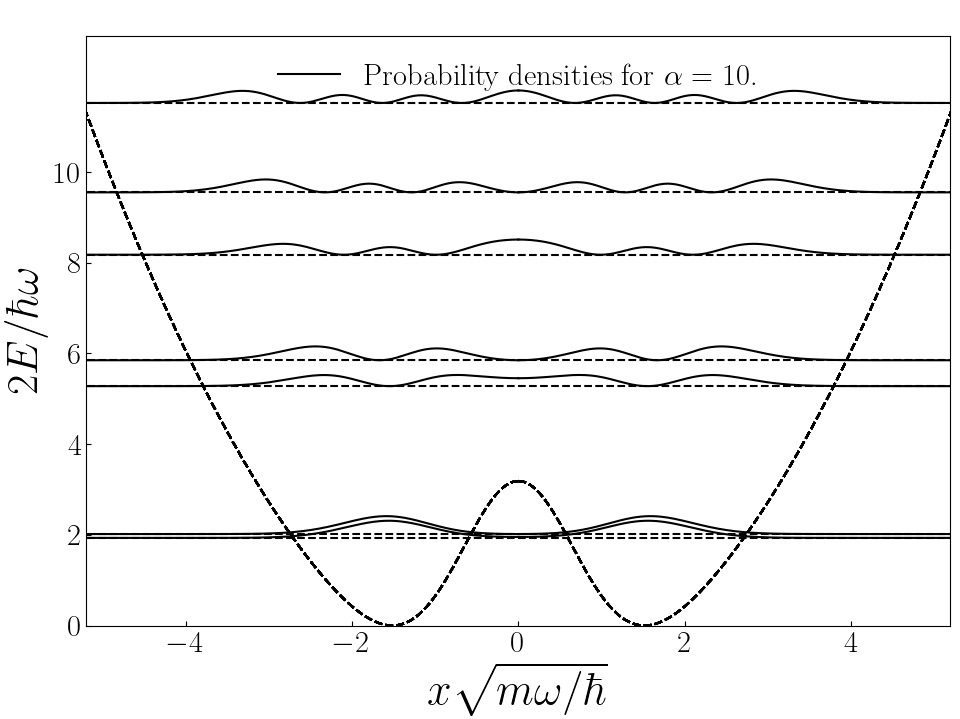
\includegraphics[scale=0.37]{alpha10_density.png}
    \caption{The first couple of probability densities for the modified harmonic oscillator with $\alpha=10$.}
    \label{4apr2029}
\end{figure}
\begin{figure}[b!]
    \centering
    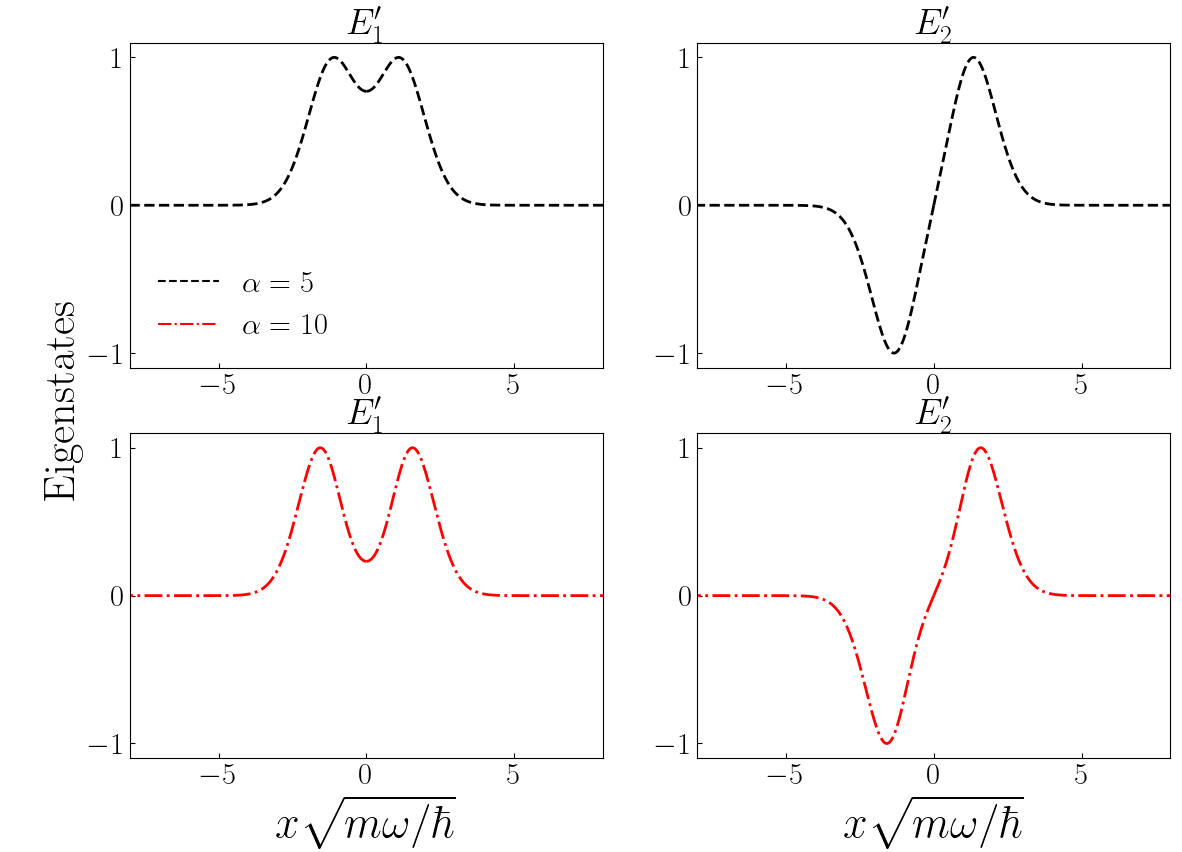
\includegraphics[scale=0.31]{first_eigenstates_alphas.png}
    \caption{The first couple of eigenstates for $\alpha=5$ and $\alpha=10$.}
    \label{5apr0727}
\end{figure}
\begin{figure}[t!]
    \centering
    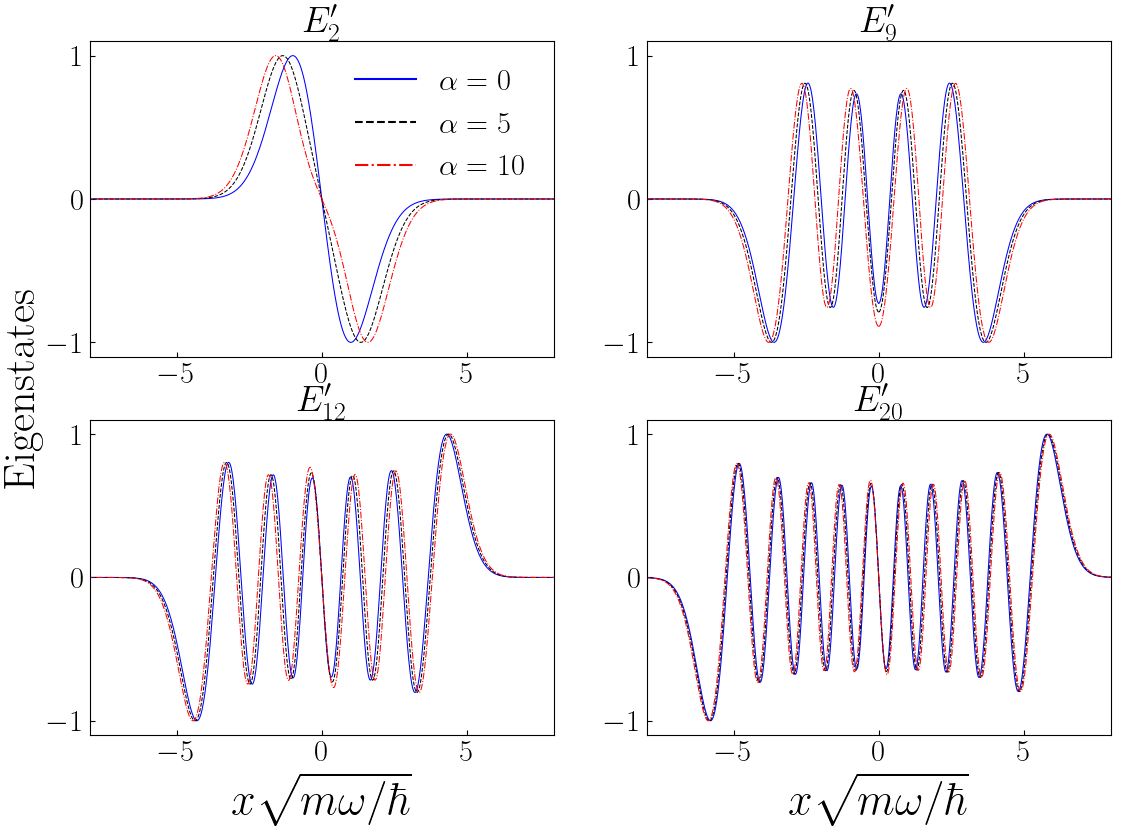
\includegraphics[scale=0.33]{high_energy_comparison.png}
    \caption{Comparison of eigenstates for different values of $\alpha$. For large energies, the eigenstates start to look like harmonic oscillator states ($\alpha=0$).}
    \label{4apr2029}
\end{figure}
%\begin{figure}
%    \centering
%    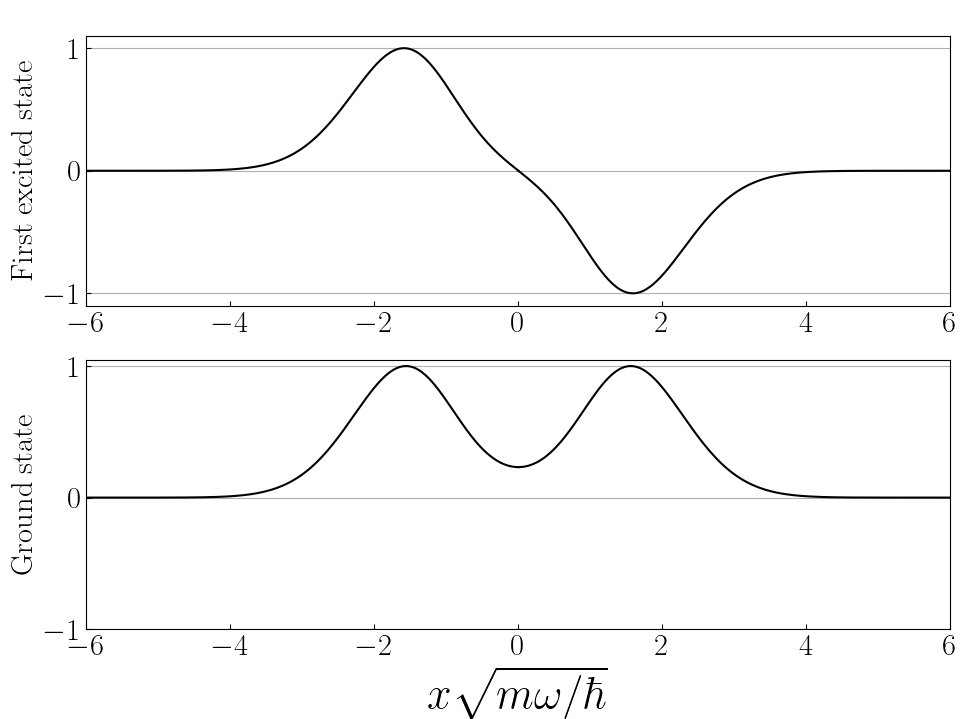
\includegraphics[scale=0.35]{first_states_alpha10.png}
%    \caption{}
%    \label{4apr2217}
%\end{figure}
\begin{figure}
    \centering
    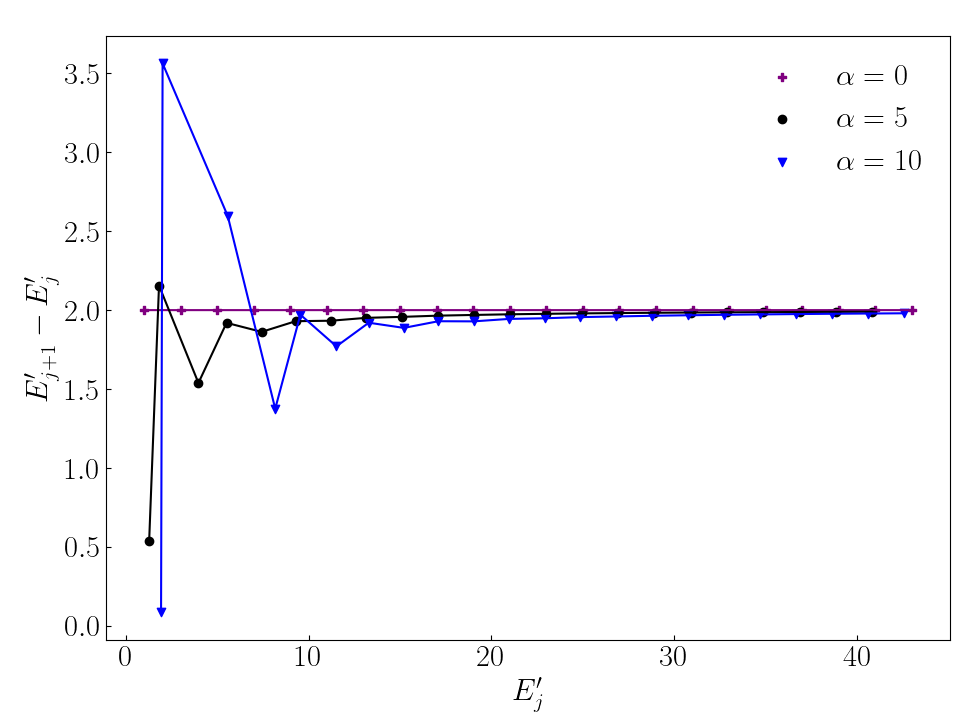
\includegraphics[scale=0.35]{relationship.png}
    \caption{The spacings between the energies for different $\alpha$. For large energies, the energy levels and the spacings between the energy levels become more similar to the harmonic oscillator ($\alpha=0$).}
    \label{4apr2044}
\end{figure}
%\begin{tabular}{c c c}
%    \centering
%    $E'$ & $|H\mathbf{u}-E'\mathbf{u}|_\text{max}$ & $h$ \\ 
%    \hline\hline \\ 
%    \,\,1.0001 & $7.57\cdot 10^{-8}$ & 0.025 \\ \ 
%    1.0031 & $3.59\cdot 10^{-8}$ & 0.25 \\ \ 
%    1.0083 & $3.77\cdot 10^{-7}$ & 0.5 \\ \ 
%    3.0000 & $3.70\cdot 10^{-6}$ & 0.025 \\ \ 
%    3.0013 & $1.59\cdot 10^{-12}$ & 0.25 \\ \ 
%    3.0316 & $4.97\cdot 10^{-14}$ & 0.5 \\ \ 
%    5.0000 & $1.55\cdot 10^{-6}$ & 0.025 \\ \ 
%    5.0005 & $1.81\cdot 10^{-12}$ & 0.25 \\ \ 
%    5.0288 & $3.41\cdot 10^{-13}$ & 0.5 \\ \ 
%    %7.0070 & $4.01\cdot 10^{-7}$ & 0.025 \\ \ 
%    %7.0070 & $3.69\cdot 10^{-13}$ & 0.25 \\ \ 
%\end{tabular}
%\subsection*{Numerical solution to eigenvalue problem}
%%We wish to solve \eqref{29mar1748} numerically by discretizing the real line and the second derivative of $u$. In order to do so, we introduce the gridpoints $\xi_j$  and the approximations of the function $u$ at these gridpoints, $u_j\approx u(\xi_j)$. Furthermore, we assume that $\xi_j\in[-L,L]$, where $L$ is chosen such that $u(\xi)\approx 0$ for $|\xi|\geq L$. Since the eigenfunctions of an even potential can be taken to be even or odd, we can focus on the interval $[0,L]$ and apply the boundary conditions 
%\begin{equation}
%    \begin{split}
%        &u'(0) = 0 \quad\text{and}\quad u(L) = 0 \quad \text{for even } u, \\ 
%        &u(0) = 0 \quad\text{and}\quad u(L) = 0 \quad \text{for odd } u.
%    \end{split}
%\end{equation} 
%The second derivative is approximated up to fourth order:
%\begin{equation}
%    \begin{split}
%        u''(x_j) &\approx \frac{1}{12h^2}\big(-u_{j-2}+16u_{j-1}-30u_j \\ 
%        &\hspace{1.7cm}+16u_{j+1}-u_{j+2}\big) 
%    \end{split}
%\end{equation}

\newpage
\null
\newpage
\subsection*{Appendix: Construction of finite difference matrices}
For the second derivative in the hamiltonian, the following difference formula was used:
\begin{equation}
    \begin{split}
        u''(\xi_j) &= \frac{1}{12h^2}\big(-u(\xi_{j-2})+16u(\xi_{j-1})-30u(\xi_j) \\ 
        &\hspace{1.7cm}+16u(\xi_{j+1})-u(\xi_{j+2})\big) + O(h^4)
    \end{split}
\end{equation}
where $h$ is the step size.
For the hamiltonian used for the odd states, $H_\text{odd}$, the boundary condition $u(0)=0$ was dealt with by using an asymteric difference formula:
\begin{equation}
    \begin{split}
    u''(h) &= \frac{1}{12h^2}\big(10u(0)-15u(h)-4u(2h) \\
    &\hspace{1.2cm} +14u(3h)-6u(4h)+u(5h)\big) + O(h^4).
    \end{split}
\end{equation}
For the even hamiltonian, $H_\text{even}$, the boundary condition $u'(0)$ was dealt with by introducing two ghost points to the left of $0$ and then using the following difference formulas to write $u(-2h)$ and $u(-h)$ in terms of $u(\xi_j)$ for $\xi_j\geq 0$:
\begin{equation}
    \begin{split}
        &u'(0) = \frac{1}{12h}\big(u(-2h)-8u(-h)+8u(h)-u(2h)\big) \\ 
        &\hspace{2.3cm} +O(h^4) \\ 
        &u'(0) = \frac{1}{12h}\big(-3u(-h)-10u(0)+18u(h) \\ 
        &\hspace{2.3cm} -6u(2h)+u(3h)\big)+O(h^4)
    \end{split}
\end{equation}
Using these difference formulas one could set up the eigenvalue problems for the different operators. 
\end{large}
\end{document}
